\section{OPQ Makai}
\label{sec:opq-makai}

\subsection{Overview}

OPQ Box provides an inexpensive hardware device for collecting four important power quality measures with high fidelity, but realizing its potential requires an innovative approach involving two-way communication between OPQ Boxes and the OPQ cloud-based services. To see why, consider the IEEE 1159 standard for single location power quality monitoring \cite{unruh_ieee_2018}.  For transient monitoring, IEEE 1159 suggests a sampling rate of at least 7680 samples/second, up to 1 Megasample/second. This implies that if the cloud service requires the high fidelity data from all OPQ Boxes, it would incur a very large bandwidth cost. At 20 Ksamples/second with 16bit samples, a single OPQ Box will generate 300Kb/second of network bandwidth. Several thousand devices would easily saturate a 1 GB network link. In addition, collecting and recording all of the raw waveform data from residential power quality meters could lead to security and privacy issues.

Network bandwidth saturation is a common problem for distributed sensor networks, and a common solution is called "self-triggering".  In this approach, each monitoring device is configured with a threshold value for one or more measures of interest. When the threshold for a measure of interest is exceeded, then and only then is data sent over the network to cloud-based services for analysis.

The problem with the self-triggering approach is that grid-wide power quality events do not affect the entire grid in the same way. For example, due to the grid’s hierarchical structure, a voltage sag on one sub-circuit can manifest as a sag of a different magnitude or even a swell on another \cite{kahle_power_2015}. This may result in a situation where some of the monitoring devices will not consider a power quality anomaly as an event, because it did not surpass the metric threshold, and simply ignore it. From an analysis perspective, however, it can be useful to get raw data from all of the affected devices, not just the ones that were the affected to the point where the box was triggered. This additional information can be used to localize the disturbance, as well as better evaluate its impact.

Since sending all the data is infeasible, and since the self-triggering approach can potentially miss important forms of information, OPQ implements a novel, hybrid centralized/decentralized data acquisition scheme which involves two-way communication between the OPQ Boxes and a cloud service called OPQ Makai. In this scheme, OPQ Boxes use local processing resources to feature extract the incoming waveforms while storing them locally for an hour. Each OPQ Box sends its feature data to OPQ Makai once a second, which we called the "triggering stream". Feature data is very small, on the order of a few kilobytes, and so this approach allows the sensor network to scale to thousands of devices with acceptable network bandwidth requirements.  OPQ Makai processes the incoming triggering stream and looks for anomalies. If an anomaly is present in only a single device, it is highly probable that the cause is local and not grid-level. On the other hand, if the triggering stream shows an anomaly temporally collocated across multiple devices, the entire network or a subset of the network may be queried for raw waveform data for a temporal region which corresponds to the disturbance in the triggering stream.

Our pilot study, discussed in Section \ref{sec:pilot-study} will provide examples of the novel analysis capabilities made possible by OPQ Box and OPQ Makai communication. In general, here are the main advantages of our hybrid centralized/decentralized approach over traditional self-triggering and the ``naive" approach of sending all of the data:

{\em Bandwidth usage is minimized.} Instead of sending the entirety of raw data, only extracted features are sent. This results in a tiny fraction of the bandwidth requirement when compared to raw waveforms. Furthermore, the temporal window which encompasses a single feature can be adjusted in real time. Thus, as soon as an anomalous behavior is observed in a subset of sensors, this window can be adjusted for a finer grained feature extraction.

{\em Effects of latency are minimized.} In this case, "latency" refers to the time required for OPQ Makai to process the incoming feature stream and decide whether to request high fidelity data from one or more OPQ Boxes. Even at 1M samples/second at 16 bits of resolution, the memory requirement to store 5 minutes of raw waveform without compression are on the order of 512MB, which is well within the realm of inexpensive single board computers such as Raspberry PI. With compression specifically suited to the signal of interest, the memory requirement can be reduced even further. In the case of the OPQ sensor network, OPQ Makai has an hour to process feature data and request high fidelity data from OPQ Boxes. During our pilot study, OPQ Makai always responded within a second or two.

{\em Cloud processing requirements are reduced.} Since feature extraction is already performed at the device level, cloud computation requirements are reduced. With the advent of the Internet of Things, the computational capacity of edge devices is increasing.

{\em Subthreshold data acquisition can improve understanding of grid-local anomalies.} OPQ Makai makes the decision to acquire raw waveform from OPQ Boxes. This allows analysis of data from devices which were only mildly affected or even not affected at all by the disturbance. This creates new possibilities for investigation of disturbance propagation across the sensed area, as will be discussed in Section \ref{sec:pilot-study}.

{\em Temporal locality allows OPQ to provide improved insights into power quality anomalies over traditional triggering algorithms.} By exploiting the idea of temporal locality, it is possible to ascertain the geographical extent of an anomaly with only coarse features. This allows for a simple robust algorithm which may be deployed at the sink node for anomaly detection.

\subsection{Design}

OPQ Makai is a distributed extensible microservice framework responsible for receiving the triggering stream from the OPQ Boxes, locating anomalous temporal regions and requesting raw waveform for the anomalous time ranges. As shown in Figure \ref{fig:makai-design}, Makai consists of four major components: Acquisition Broker, Triggering Broker, Event Service and the Acquisition Service.

\begin{figure}
\center 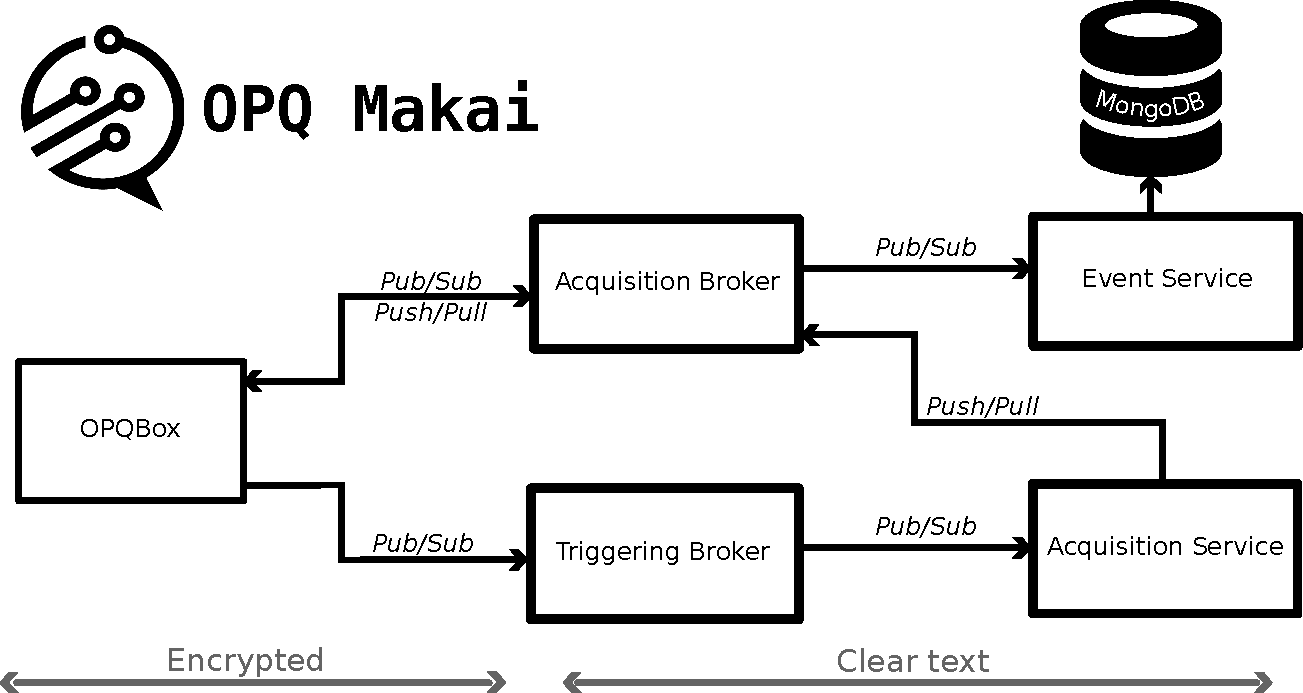
\includegraphics[width=3in]{images/makai/makai_main.pdf}
\caption{Makai component design}
\label{fig:makai-design}
\end{figure}

The Triggering Broker is perhaps the simplest component of the OPQ Makai system. The triggering stream generated by the OPQ Boxes is encrypted to preserve user privacy. In order to minimize the CPU time spent decrypting the data across multiple OPQ services, the Triggering Broker decrypts the data and sends clear text measurements to other OPQ cloud services. The Triggering Broker uses the ZeroMq subscribe socket to receive data from OPQ Boxes, and sends it via a publish socket to any connected client. Each publish message is published to a topic which corresponds to the ASCII representation of the originating OPQ Box ID. This allows services which utilize the Triggering Broker to select a subset of IDs to operate on. This is useful for load balancing the backend services, or dividing the OPQ network into separate regions with no electrical connections between them.

The Acquisition Broker manages the two-way communication between the OPQ Boxes and the rest of the cloud infrastructure. Unlike the triggering stream which originates from the OPQ Box, two-way communication is always initiated by OPQ cloud services. Two way communication is realized via a command response interface, where the OPQ service initiates the communication by sending a clear text command to the Acquisition Broker, which then forwards it in encrypted form to the appropriate OPQ Boxes.

The Acquisition Service resides between the Triggering and Acquisition Brokers. The Acquisition Service is responsible for three tasks:
(1) Computation of statistics of the incoming triggering stream; (2) Hosting plugins for triggering stream analysis; and (3) Generating data event requests for OPQ Boxes. The Acquisition Service accesses the triggering stream by connecting to the publish socket of the Triggering broker. Since the connection is managed through the ZeroMq publish-subscribe socket, several Acquisition Services can be connected to a single Triggering broker endpoint, each servicing a subset of OPQ Boxes by subscribing to only specific devices. The Acquisition Service does not include any analysis capabilities by default. Instead, analysis is performed by shared library loadable plugins. These plugins can be loaded and unloaded at runtime, thus allowing live upgrading and testing of new analysis methods.

The Event service is a microservice which stores raw data generated by OPQ Boxes in the MongoDB Database. On initialization, the Event service queries MongoDB database for the highest event number recorded so far, connects to the Acquisition Broker’s publish port, and subscribes to all messages that start with the prefix ``data”. This allows the Event service to capture every response from OPQ Boxes generated from commands issued by the Acquisition service plugins. Once the Event service receives a data response with an identity containing an event token it hasn’t seen before, it will increment the event number, and store it in an internal key value store.


